\section{Study Design and Methods}
\label{sec:methods}
\subsection{Overview and units of observation}
Figure~\ref{fig:overview} summarizes the implemented process. We first construct requests associated with a topic and a desired semantic destination, then measure the resulting text with frozen external embedding maps. For each execution condition, the generator formulates search queries and receives selected evidence from an immutable snapshot. It returns an answer and an ordered subset of evidence identifiers. Separate judgments assess relevance to the request and support for the completed answer.

A \emph{topic} is the dataset's keyword grouping, such as ``robinhood vs etrade.'' An \emph{information need} is the underlying question or practical objective a person wants to resolve; its count cannot be inferred from the number of topics. A \emph{prompt variant} is one retained request string associated with a topic. Variants may change purpose as well as wording, and have not been verified as meaning-preserving paraphrases of one base question. A \emph{search query} is an intermediate string generated for retrieval. An \emph{execution cell} is a prompt paired with a generator, engine snapshot, strategy, and recorded evidence condition. An \emph{answer} is the resulting text. A \emph{source} is an identified URL with the exact title and snippet text supplied as evidence, not a fetched full document. A \emph{judgment} is a separate evaluation of one cell or one source within it. These units have different denominators.

\begin{figure*}[t]
\centering
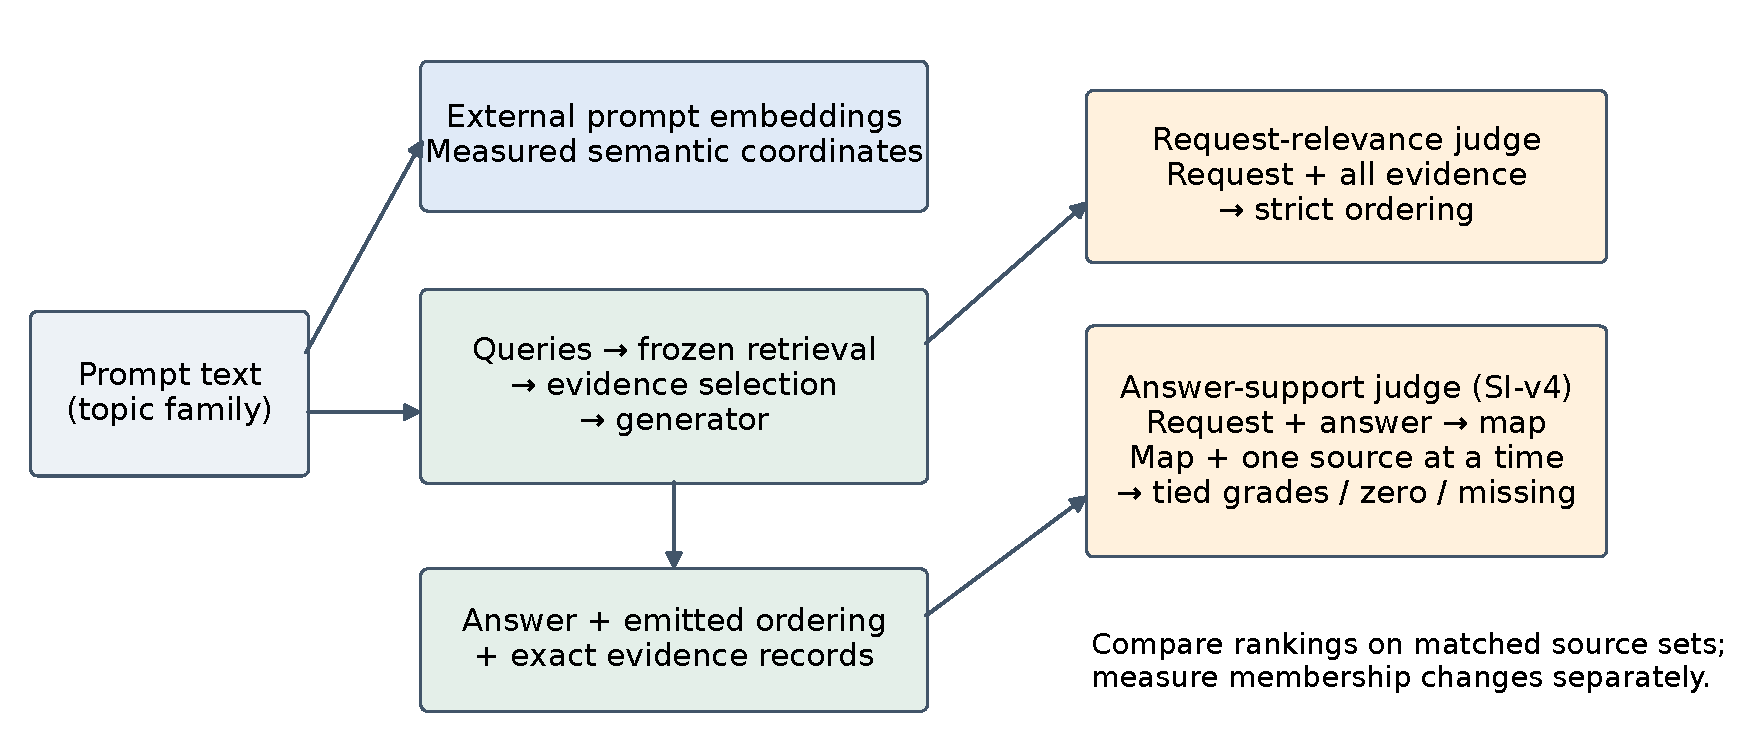
\includegraphics[width=\textwidth]{figures/study-overview.pdf}
\caption{Implemented measurement paths. Prompt embeddings describe request text; they are not hidden states of the answer generator. Local retrieval and evidence selection can change the source set across prompts. The relevance judge sees the request and all candidate evidence, but no answer. The support procedure first maps the completed answer without sources, then assesses each source separately. The diagram specifies inputs and outputs, not observed ranking effects or validation of the judgments.}
\label{fig:overview}
\end{figure*}

\subsection{A real running example}
\label{sec:example}
Table~\ref{tab:example} shows three actual prompts from one topic. We selected the illustrated execution by taking the lexicographically smallest natural-condition cell identifier in the saved 40-cell support-development audit, rather than selecting for a particular score. The other two prompts are retained variants from the same topic that illustrate different measured positions. This is a transparent illustration, not a representative sample of effects.

\begin{table*}[t]
\small
\begin{tabularx}{\textwidth}{@{}lYrrr@{}}
\toprule
 & Verbatim retained prompt & Intended & Measured & Measured\\
 & & target & axis 1 ($z$) & percentile\\
\midrule
A & What are the fundamental structural differences in how the platforms operate when looking at robinhood vs etrade? & .029 & $-1.688$ & .021\\[3pt]
B & I’m trying to transfer my investments this afternoon — what exact steps do I need to follow to set up a full transfer between robinhood vs etrade? & .924 & $-.329$ & .586\\[3pt]
C & Set up and verify same-day stock transfer from Robinhood to E*TRADE with account confirmation steps & .885 & .497 & .921\\
\bottomrule
\end{tabularx}
\caption{Real prompt-family illustration. The intended target is a construction instruction; the measured $z$ coordinate comes from the final aligned embedding maps; the percentile is the rank within the 26,009 retained strings. These are different scales. Only B's execution is inspected here: Llama, Reactive Loop, DuckDuckGo snapshot, natural evidence condition. Its saved generator ordering is Benzinga $\succ$ The Smart Investor $\succ$ Investopedia. All three historical SI-v3 support grades are zero. Request-relevance rankings, SI-v4 grades, and A/C execution comparisons remain \textbf{TODO}; no corresponding permutations are inferred.}
\label{tab:example}
\end{table*}

For prompt B, the generator was supplied with three snippets comparing the two platforms. The Benzinga snippet contrasts commission-free trades and a beginner-friendly app with research tools and a broader product range. The Smart Investor snippet contrasts ease of use with a more versatile trading environment; the Investopedia snippet also compares trading and resources. These snippets do not themselves present the transfer procedure requested. The saved generator list places Benzinga first, followed by The Smart Investor and Investopedia.

The answer begins: ``To set up a full transfer between Robinhood and E*TRADE, follow these steps: 1) Log in to your Robinhood account and go to the `Transfers' or `Account' section.'' It continues with a transfer procedure. This is quoted output, not verified financial guidance. The historical support judge assigned all three sources grade zero. Consequently there is no positive-support top source in this record, and top-source agreement with support is undefined. Treating the listed order as a support ordering, or arbitrarily putting the three zero-score sources into a strict bottom order, would create information that the judgment does not contain.

The example's intended target of .924 also differs from its measured percentile of .586. Percentiles and construction targets use different reference scales; this difference alone is not evidence of an acceptance failure. The illustration establishes the distinction between the measurements, not that more action-ready prompts generally have lower support. Appendix~\ref{app:example} records identifiers and provenance limits; Appendix~\ref{app:example-full} reproduces the answer and snippets. \todo{Complete this same example with verified relevance and SI-v4 outputs, and retrieve the corresponding executions for A and C without substituting illustrative rankings.}

\subsection{Dataset provenance and construction}
\label{sec:population}
The topic inventory contains 1,011 keyword groups. \todo{Recover the original keyword acquisition source, collection dates, licensing, language/domain composition, and mapping from topics to independently assessed information needs.} The earlier manuscript's dataset description is not sufficient provenance for the present retained population. A topic shared by requests for explanation and execution does not make those requests one independent question.

Prompt generation used Qwen3-32B and Gemma-4-31B-it with versioned instructions. The construction plan specified 30 semantic targets per topic, giving 30,330 topic--target slots, with four candidate proposals per generation task in the initial plan. The initial design used support-aware continuous targets, while later records contain axis-1 lattice targets and additional recovery rounds. We do not describe all rounds as one uniform grid. \todo{Reconcile the target-design chronology and per-round generation settings from their pinned manifests.}

The final text contract, \code{search-trigger-v2}, permits questions, imperative requests, and concise search phrases of 4--60 words on one normalized line. Topic metadata binds a candidate to its topic; the literal keyword string and standalone interpretation are optional. Generation instructions describe semantic destinations with verbal anchors, vary surface realization, and include feedback from earlier measured candidates. A recovery profile for high-axis targets asks for action-enabling requests without pretending that the search system has performed an action. Exact instructional templates and their dynamic substitutions appear in Appendix~\ref{app:templates}.

Quality checks combine mechanical text checks, independent model review, embedding measurements, and selection constraints. Under the final review contract, a candidate must be topical, express search intent, be web-answerable and natural, and receive at least 4/5 relevance. The strict selection check requires agreement with its target within .035 on normalized axis 1 under both frozen embedding views. Axis 2 is measured but is not that acceptance gate. Selection enforces one-to-one topic/target assignments and uniqueness of delexicalized templates, alongside a diversity gate. These are automated checks; they do not prove that all variants are distinct information needs or that people would issue them naturally.

The merged-candidate summary records 1,314,060 candidate records and 1,296,908 accepted records. The supporting summaries use different acceptance labels for the latter count, so we do not reconstruct a fine-grained filtering waterfall from them. The final files themselves contain 26,009 distinct strings and candidate identifiers, with exact text-hash joins to 26,009 measured-coordinate records. Qwen generated 13,515 retained strings and Gemma generated 12,494. Topics contain between 18 and 30 retained prompts. Table~\ref{tab:counts} distinguishes these direct file checks from manifest-level counts.

Retained-slot coverage is 26,009/30,330, or 85.75\%. It measures filled planned topic--target slots, not coverage of independent information needs, the web, or downstream executions. The saved selection summary leaves 4,321 slots unresolved. Its diversity gate passes, but its spacing gate and full-target-population verification do not. A passing final text-compliance audit must therefore not be described as a completely filled or evenly spaced design.

Prompt selection was iterative and used semantic feedback. \todo{Verify the provenance chronology needed to state whether any prompts, filtering thresholds, or semantic maps were tuned after inspecting downstream ranking results; absence of such tuning has not been established.} The final population is frozen for the executions described here, but freezing does not retrospectively establish independence from earlier development choices.

\begin{table*}[t]
\small
\begin{tabularx}{\textwidth}{@{}p{.28\textwidth}rY@{}}
\toprule
Unit or stage & Count & Evidence and interpretation\\
\midrule
Keyword topics & 1,011 & Counted in final prompt records; independent information needs unknown.\\
Planned topic--target slots & 30,330 & Construction manifest; 30 requested targets per topic.\\
Merged candidate records & 1,314,060 & Saved summary; raw merged archive not reread for this draft.\\
Accepted candidate records & 1,296,908 & Summary count; exact stage labels require reconciliation.\\
Retained prompt strings & 26,009 & Rehashed final file; all unique; 18--30 per topic.\\
Exact prompt--coordinate joins & 26,009 & Candidate IDs and UTF-8 text hashes verified.\\
Unresolved target slots & 4,321 & 14.25\% of intended slots; spacing gate did not pass.\\
\midrule
Full factorial target per generator & 312,108 & 26,009 prompts $\times$ 2 strategies $\times$ 2 engines $\times$ 3 recorded conditions.\\
Full target across two generators & 624,216 & Planned cells, not completed answers or support-judge calls.\\
Llama registry planned cells & 310,380 & Published registry; 1,728 fewer than full per-generator target.\\
Llama recorded completed / failed & 310,374 / 6 & Registry and bundle audit; payload rows not fully reread.\\
Qwen published completed cells & 24,218 & Audited JUPITER bundles only; not total cross-cluster completion.\\
Historical support-development cells & 40 & 40 prompts; 214 source tasks, two repetitions, SI-v3.\\
Final matched relevance/SI-v4 cells & \textbf{TODO} & No verified completed population export located.\\
\bottomrule
\end{tabularx}
\caption{Design and evidence counts. Prompt counts come from direct final-file checks; execution counts describe the publication audit at 2026-10-01 05:26:47 UTC, not live cluster state. Completed registry entries do not establish answer quality, usable rankings, or valid support judgments. The three historical evidence conditions are retained strata, not separate research questions. Per-model/engine/strategy completion and analysis-eligibility denominators remain to be verified.}
\label{tab:counts}
\end{table*}

\subsection{Measuring prompt semantics}
\label{sec:semantics}
We distinguish an \emph{intended destination}, supplied to prompt generation, from a \emph{measured position}, computed from the resulting text. The measurement uses two external LLM2Vec encoder views based on Qwen3-8B and Mistral-7B-Instruct-v0.2. It does not extract hidden states from the answer generator. Base-model revisions appear in Appendix~\ref{app:config}; exact encoder-adapter revisions still require a complete record.

The frozen map code normalizes each embedding and fits a ridge prediction of a model-consensus readiness label. It also fits rubric dimensions describing reversed information seeking, evaluation, selection commitment, and action implementation. A singular-value decomposition of their coefficient matrix supplies two supervised directions. The scalar predictor and the first supervised direction are related summaries, but they are not the same measurement. The aligned views yield the saved consensus axis-1 coordinate used in the worked example. The final map also reports a rank percentile within the retained population. This percentile preserves order but does not make semantic distances equally spaced or represent a probability of action.

A frozen calibration report contains 4,519 usable development items and 3,570 usable confirmation items. Scalar-prediction Spearman correlations with model-consensus labels are .680 for the Qwen view (saved 95\% interval [.661, .698]) and .732 for the Mistral view ([.717, .746]). The saved intervals use 1,000 bootstrap resamples of confirmation rows, with fixed predictions; they do not refit the encoders or account for dependence among related prompts. These are construct checks against model judgments, not validation against human intent or behavior. \todo{Verify encoder adapters, calibration-item provenance, label-judge identities, exclusion counts, and the consequences of related prompts for these row-resampled intervals.} Agreement between the two views in the selected population is additionally conditioned on selection that already required their agreement.

Figure~\ref{fig:geometry} characterizes the retained population without claiming a ranking result. A broader semantic-neighborhood analysis would compare distances between the external prompt embeddings; a one-dimensional coordinate can only characterize one direction within that space. The saved permutation-analysis code implements separate directional fits, and does not establish the full-space neighborhood relationship in RQ1.

\begin{figure*}[t]
\centering
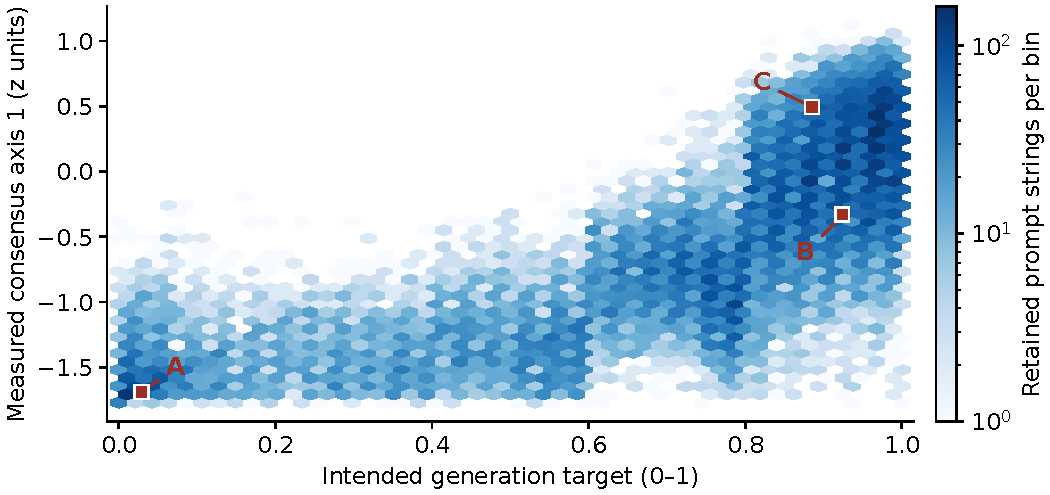
\includegraphics[width=.88\textwidth]{figures/target-measurement.pdf}
\caption{Construction targets and measured positions for all 26,009 retained prompt strings. Each hexagonal bin counts exact prompt--coordinate joins; color shows count on a logarithmic scale. The vertical coordinate is the final consensus axis-1 $z$ value, not a probability or a generator hidden state. A, B, and C identify the real variants in Table~\ref{tab:example}. This is a descriptive population census, so no sampling interval is drawn. It characterizes the selected population and the distinction between scales; it does not estimate semantic-to-ranking association or validate the intended target scale.}
\label{fig:geometry}
\end{figure*}

\subsection{Search, evidence selection, and generation}
\label{sec:generation}
The implemented engines are immutable snapshots of DuckDuckGo and SearxNG search results. For a generated query, the local adapter prioritizes exact keyword/query matches, then lexical overlap, stored engine position, a deterministic query--URL hash, and original row index. It returns at most 20 records per search action. A cross-encoder scores candidates for evidence selection. We use \emph{compaction} to mean this selection of a smaller evidence set; it must not be confused with silently shortening every snippet to a specified token count.

Parallel Expansion generates three distinct search queries, retrieves their results, deduplicates by URL, scores the combined records against the original request, and retains up to seven. Reactive Loop starts with search and permits up to three search actions. Each action retains up to three results scored against the current search query; accumulated observations are deduplicated by URL. The model may finish after observing evidence, or must finish when the action budget is exhausted. The distinct query used for compaction is part of the strategy difference. The pseudocode gives the conceptual procedure; Appendix~\ref{app:templates} contains the literal instructions.

\begin{figure}[t]
\small
\fbox{\begin{minipage}{.94\columnwidth}
\textbf{Parallel Expansion}\par
1. Generate three queries from the request.\par
2. Retrieve up to 20 records per query.\par
3. Merge records; deduplicate by URL.\par
4. Apply recorded evidence-condition hook.\par
5. Score against request; retain top seven.\par
6. Generate answer and evidence-ID ordering.\par\medskip
\textbf{Reactive Loop}\par
1. Start with no observations; require search.\par
2. For at most three search actions:\par
\hspace*{.6em}a. Generate query from request/observations.\par
\hspace*{.6em}b. Retrieve up to 20; apply condition.\par
\hspace*{.6em}c. Score against query; retain top three.\par
\hspace*{.6em}d. Accumulate deduplicated observations.\par
\hspace*{.6em}e. Allow finish after observing evidence.\par
3. Force finish when search budget is exhausted.\par
4. Return answer and evidence-ID ordering.
\end{minipage}}
\caption{Strategy pseudocode. Retrieval uses frozen snapshots. The condition hook records existing natural, ablated, or shuffled strata; those controls are not new research questions. Output validation and bounded repair are described in the text. Budgets count search actions and source records, not answer tokens.}
\label{fig:pseudocode}
\end{figure}

The answer generator sees the request and evidence records containing identifiers, URLs, titles, and snippets. It does not receive measured coordinates. Intermediate prompts expose accumulated observations, rather than a fetched full web page. The final output contains an answer and a ranking of supplied evidence identifiers, possibly a subset. The controller checks format and membership and records repair and truncation events. Its answer-length contract is 1,200 Python characters, separate from model output-token limits. Some support-preparation paths recover a longer answer from an exact matching trace when the stored answer is a truncated prefix. The analysis must therefore distinguish the answer stored for generation from the text actually judged. \todo{Report counts of repair, prefix recovery, truncation, unresolved source references, and exclusion by execution condition.}

The recorded generator families are Qwen3.8-27B and Llama-4-Scout-17B-16E-Instruct. The current Qwen bout configuration caps query output at 256 tokens and final output at 2,048 tokens; the inspected Llama adaptive configuration uses 256 and 4,096. Histories include budget changes, so these settings cannot be assigned to every historical cell. \todo{Join each execution to its pinned configuration, decoding settings, template hashes, and model revision before producing condition-level comparisons.} The cross-encoder is BAAI/bge-reranker-v2-m3; its pinned revision and documented settings appear in Appendix~\ref{app:config}.

The global snapshot is fixed, but candidate membership is \emph{not guaranteed fixed within a topic family}. Different generated queries can retrieve and select different records. An identical URL can also be paired with different evidence text. An ordering-only comparison requires matching source identity, title, text, and relevant presentation/configuration fields. Where pools differ, the records support a membership comparison and, separately, an ordering comparison on shared sources; the latter cannot describe excluded sources.

Historical natural, ablated, and shuffled conditions remain metadata strata. Their purpose and scope are documented with the configuration, but this manuscript asks no source-removal or input-order question. The shuffle hook precedes score-based compaction, so downstream sorting can undo a nominal shuffle. We do not interpret that label as proof that the generator received a different order. \todo{Audit effective presentation sequences and freeze which recorded strata enter each main comparison.}

\subsection{Obtaining relevance and answer-support orderings}
\label{sec:judges}
\paragraph{Request relevance.}
The implemented relevance judge receives the request and every evidence record supplied to that judging task, including URL, title, and snippet, but no generated answer. It must return each evidence identifier exactly once, from most to least useful for answering the request. This produces a strict judge-derived ordering. The schema calls it \code{ideal_relevance_ranking}; we use \emph{request relevance} because a judge output is not a verified ideal or human gold standard. The format cannot express ties and therefore imposes an order even when sources appear equally relevant. The Nemotron judging configuration identifies NVIDIA-Nemotron-3-Nano-30B-A3B-BF16. \todo{Verify completed relevance exports, exact per-run judge configuration, and an independent assessment of ranking quality.}

\paragraph{Textual support for the completed answer.}
A source can address the request without supporting the answer the generator chose to write. The current support-development procedure first constructs a source-blind map of the answer, then evaluates each source against that fixed map. The implementation is named \emph{Source Importance version 4} (SI-v4). Its purpose is to avoid conflating topical relevance, answer quality, and support for the answer as written.

In Stage A, the judge sees the request and the citation-masked complete answer, with indexed original word spans and no sources. It identifies assertions, recommendations, attributed reports, and claims about absence of information across the entire evidence set. It assigns each substantive claim an importance role within that answer: central, major, secondary, or peripheral. Every word must belong to a claim span or an explicit exclusion. Preserving words and accounting for spans are mechanical checks; neither proves that the map preserves meaning or importance.

In Stage B, the judge sees the same request and answer, the fixed map, and one unchanged source title/text record. It sees no source URL, other sources, generator identity, generator ordering, readiness value, or evidence-condition label. It identifies full or partial support, contradiction, or genuine uncertainty, with one to three representative source-passage witnesses per finding. The ordinal grade ranges from 0, no identifiable substantive support, to 5, support for most of the answer's essential content. Intermediate grades distinguish peripheral, secondary, substantial, and central supported content. The grade concerns importance \emph{within the completed answer}, including an off-target answer; it is not a relevance score, a fraction of claims, or a test of factual truth. Redundant sources may receive the same grade.

Uncertainty and map issues produce a missing grade, not zero. An unusable map blocks dependent scoring; a map flagged downstream prevents treating the cell as cleanly scored. Pure abstention and answers consisting only of global-absence claims can be ineligible for source-level scoring. One source cannot establish that information is absent from all sources. These cases require distinct denominators rather than being merged with unsupported but assessable answers.

Positive support grades form descending tied groups. Zero-grade sources are recorded separately and remain unranked in the positive-support ordering. Missing grades invalidate complete-cell metrics. When every score is zero, the positive top group is empty and top-source agreement is undefined; when grades are constant, a correlation needing grade variation is undefined. Grade zero must not be converted into missing data, and missing data must not be imputed as zero. The running example illustrates the all-zero case using historical SI-v3 judgments. It does not validate SI-v4.

\subsection{Semantic and ranking comparisons}
\label{sec:analysis}
The core descriptive question is whether prompts that are close in meaning have similar orderings when comparison is possible. We first distinguish equal evidence sets from unequal sets, then identify whose orderings are compared. A permutation comparison is meaningful only over specified candidates. The implemented agreement summaries include exact ordering agreement, first-source agreement, top-$k$ overlap, and Kendall agreement on sources common to both lists. The top-$k$ code uses the smaller of three and the two list lengths. Fewer than two common sources makes common-source Kendall agreement undefined. These summaries cannot turn source absence into a lower rank.

Let $p$ denote a request and $e(p)$ its unit-normalized external text embedding. Cosine distance, $1-e(p)^\top e(q)$, describes semantic separation of two requests $p$ and $q$ in that encoder view. Let $C(p)$ be the exact evidence records for a cell and $\pi(p)$ a specified ordering over those records. These symbols do not imply that the generator, relevance judge, and support judge share an ordering or that every support output is a strict permutation. \todo{Provide the verified local-neighborhood analysis, including encoder view, distance/neighbor rule, pool-matching criteria, overlap denominators, and eligible prompt-pair counts. No such population result is established by the saved directional fitter.}

For directional analysis, the existing exploratory implementation fits a regularized Bradley--Terry model within matched comparison strata. Each source has an intercept describing its baseline position and a slope describing how its relative preference changes with a measured semantic coordinate. Let $x$ be the measured coordinate standardized using training prompts within the fitted stratum. The utility of source $s$ is
\begin{equation}
 u_s(x)=\alpha_s+\beta_s x,
\label{eq:utility}
\end{equation}
and the fitted probability that $s$ precedes $t$ as
\begin{equation}
 \Pr(s\succ t\mid x)=\sigma\bigl(u_s(x)-u_t(x)\bigr),
\label{eq:bt}
\end{equation}
where $\sigma$ is the logistic function. This probability summarizes observed pairwise orderings under the model. A slope is not a causal effect of readiness or evidence of a model's internal ranking mechanism.

The fitter standardizes the axis using training prompts only and gives each task equal total weight across its observed source pairs. Missing candidates are not converted to pairwise losses. It compares the directional fit with an intercept-only baseline on held-out log loss, Brier score, and pairwise accuracy. Default settings require six distinct training questions and two test questions within a matched stratum, with ridge penalty 1. A deterministic text-hash split keeps identical text out of both partitions, but does not by itself separate semantically similar variants or independent information needs. Separate fits for separate coordinates do not amount to a joint model of the full semantic space.

Matched strata preserve exact evidence, configuration, presentation, and ranking-length requirements. The code separates fixed-pool direct reranking from agentic retrieval. Its reports carry \code{scientific_result=false}; no verified fixed-pool result was located for this draft. \todo{Supply the eligible-stratum inventory, fitted outputs, exclusion reasons, split assignments, and sample sizes before claiming directional ranking changes.}

Pooled metrics in the existing exploratory report are unweighted means over valid comparison rows, with a separate valid-row denominator for each metric. They are not automatically averages giving equal weight to every topic, model, or engine. Pair-weight normalization inside a fit is different from pooling across fits. The current fitter supplies no uncertainty intervals. \todo{Document the final pooling population, weights, dependency-aware uncertainty procedure, and direct comparisons across conditions; do not infer a difference merely because one estimate is significant and another is not.}

RQ2 requires relevance and support outputs joined to the same request, answer, and evidence. The existing support cell-metric function compares the \emph{generator} list with support grades; it is not already a relevance-versus-support analysis. Tied support can be compared with a strict relevance order using a tie-aware measure only when grades and candidate coverage make it defined. \todo{Verify the RQ2 join and specify each comparison's handling of positive grades, zero grades, ties, missing values, and all-zero cells. Report the unranked zero set separately from any full-vector rank correlation.}
